\chapter{Low numeric precision convolution neural network}
\label{ch:low prec NN}


In this chapter, we go through the basic of convolution neural network, the mindset behind choosing linear quantization scheme, an algorithm for training a ultra-low precision neural network on large-scale dataset and finally a tensor re-pack method for deploying the network on a processor supporting low-precision MAC operation.
\section{Convolutional Neural Networks}
A typical convolution neural network layer takes a 3D \textit{input tensor} and a \textit{filter tensor}, and performs 2D convolution, producing a 3D \textit{output tensor}.It is essentially summing up \textbf{C} channel of 2D convolution for one output pixel as shown in \autoref{fig:conv_1}, this process is repeated for \textbf{M} number of filter, resulting in output tensor of \textbf{M} number of channel. 
In \autoref{fig:conv_2} shows a common techniques \textit{batching}, taking multiple input tensor and perform convolution on them at the same time; the picture also provides an example of the shape parameter \textbf{U}.
\begin{figure}
    \centering
    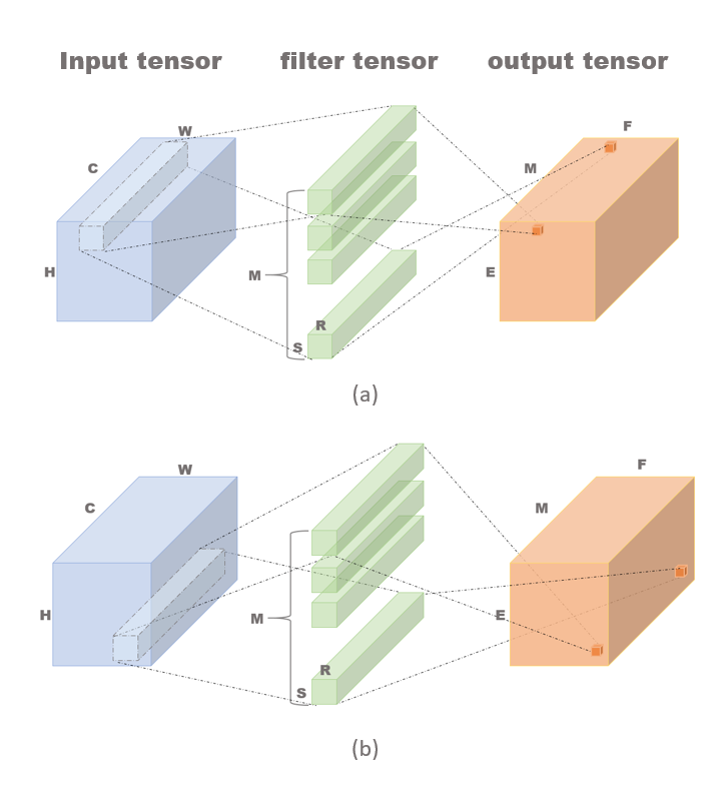
\includegraphics[width=1\linewidth]{inc/3_low_numeric_convolution_neural_network/figure/convolution_1.png}
    \caption{Computation of a convolutional layer.}
    \label{fig:conv_1}
\end{figure}
\begin{figure}
    \centering
    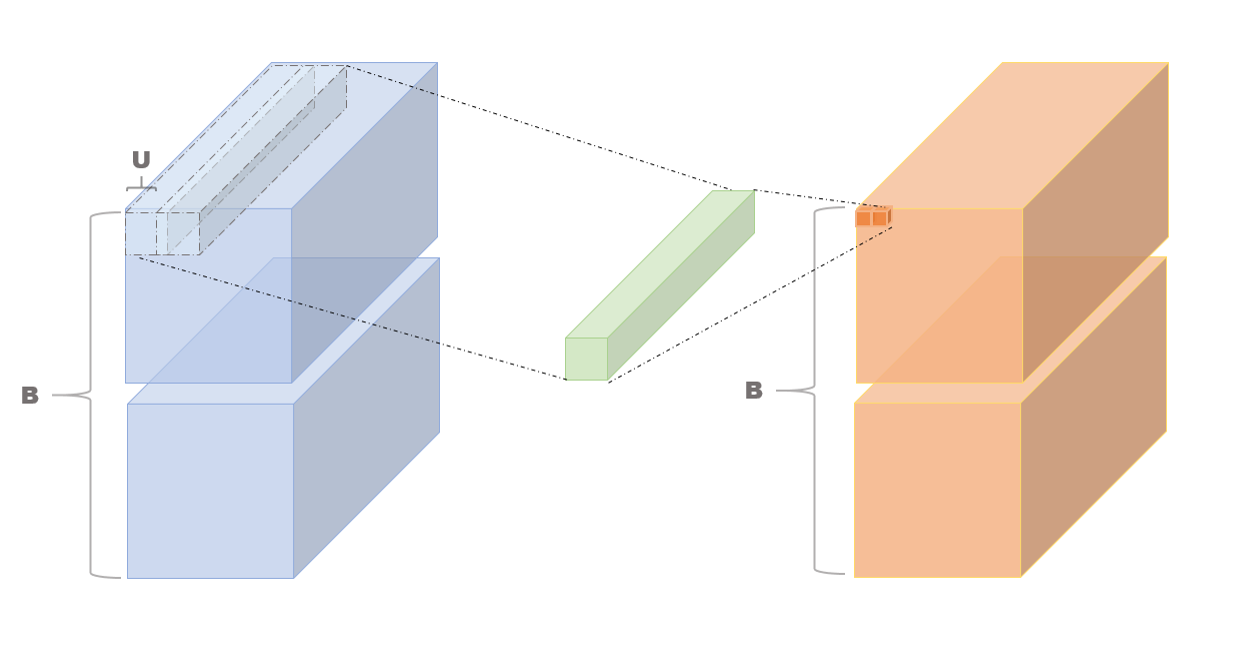
\includegraphics[width=1\linewidth]{inc/3_low_numeric_convolution_neural_network/figure/convolution_2.png}
    \caption{Shape parameter B and U.}
    \label{fig:conv_2}
\end{figure}
The entire process is formulated by \autoref{eq:conv}:
\begin{equation}
    \begin{aligned}\label{eq:conv}
    \boldsymbol{O}[z][u][x][y]=\text{ReLU}\,(
        \sum^{C-1}_{k=0}\sum^{R-1}_{i=0}\sum^{S-1}_{j=0}\boldsymbol{I}[z][k][Ux+i][Uy+j]*\boldsymbol{W}[u][k][i][j]
    ), \\
    0\leq z\leq B\ , 0\leq u\leq M\ , 0\leq y\leq E\ , 0\leq x\leq F, \\
    E=(H-R+U)/U,\,F=(W-S+U)/U
    \end{aligned}
\end{equation}


\begin{table}
    \caption{Basic shape parameters of a CNN layer}
    \label{tab:cnn_shape}
    \centering
    \footnotesize 
        \begin{tabular}{cc}
        \toprule
        Parameter & Description \\
        \midrule
        H/W & Input feature map spatial dimensions\\
        E/F & Output feature map spatial dimensions\\
        R/S & Filter spatial dimensions\\
        C & Input channels\\
        M & Output filters\\
        U & Convolution stride\\
        B & Batch,\# of feature maps to be processed\\
        \bottomrule
        \end{tabular}
\end{table}


 
\section{Low Precision CNN}
By choosing linear quantization regular multiplier and adder can be used unlike the need of look-up table in non-linear quantization. As mention briefly before, the main benefit of quantization is reduction in memory transaction, especially off-chip DRAM access. We will show in \autoref{ch:results} that given the same dataflow, 8-bit quantized model off-chip memory access wins over 16-bit model compressed with \textit{running length coding} with data sparsity of more than 70\%, indicating that quantization is a reliable compression scheme independent of sparsity of the data. This sums up our reasons behind choosing linear quantization. \\
Low numeric precision data in this work is applied to each type of tensors. Given a quantization bit $\boldsymbol{k}$, clipping threshold $\boldsymbol{\tau}$, tensor $\boldsymbol{D}$, the quantized tensor $\boldsymbol{D_q}$ is given by \autoref{eq:quant}:
\begin{equation}
    \begin{aligned}\label{eq:quant}
        \boldsymbol{D_q}=
        \textit{round}\ (\ \frac{2^{\boldsymbol{k}-1}}{\boldsymbol{\tau}}*\textit{clip}\ (\boldsymbol{D},\boldsymbol{\tau})
        \ ) \\
        \textit{clip}(\boldsymbol{D},\boldsymbol{\tau})=\begin{cases}
            \boldsymbol{D} &\|\boldsymbol{D}\|<\boldsymbol{\tau} \\
            \textit{sign}(\boldsymbol{D})*\boldsymbol{\tau} &\text{otherwise}
        \end{cases} \\
    \end{aligned}
\end{equation}
Where \textit{round}() round the number to the nearest integer. The convolution on the original tensor can therefore take the following form \autoref{eq:quant_conv}:
\begin{equation}
    \begin{aligned}\label{eq:quant_conv}
        \boldsymbol{O}\approx\boldsymbol{I}\star\boldsymbol{W}= \boldsymbol{I_q}\star\boldsymbol{W_q}
        \ \frac{\boldsymbol{\tau_I}}{2^{k_I-1}}
        \ \frac{\boldsymbol{\tau_W}}{2^{k_W-1}}
        =\boldsymbol{O_q}\  \frac{\boldsymbol{\tau_O}}{2^{k_O-1}} \\
        \boldsymbol{\alpha}\boldsymbol{I_q}\star\boldsymbol{W_q}=\boldsymbol{O_q}
    \end{aligned}
\end{equation}
\begin{equation}
    \begin{aligned}\label{eq:scalar_approx}
        \boldsymbol{\delta}=\textit{ round} ( log_2\alpha)\quad
        \boldsymbol{\gamma}=\textit{ round}( \frac{\alpha}{2^{\delta}})\quad
        \boldsymbol{\alpha}\approx=\delta\gg\gamma
    \end{aligned}    
\end{equation}
We see the part $\boldsymbol{I_q}\star\boldsymbol{W_q}$ is the low precision convolution fit for specially designed processor. $\boldsymbol{\alpha}$ merges the rest of the equation to a scaling factor, which in practice can be approximated together with other scaling factor with a 16-bit fixed-point multiplier $\boldsymbol{\delta}$ and a shifting factor $\boldsymbol{\gamma}$, see \autoref{eq:scalar_approx}. \\
The training of low precision neural network follows that of \cite{XnorNet}. See \autoref{alg:NN_train}; at training, the quantized convolution results are fed forward through the network, error is computed based on the quantized value, and the gradient is back-propagated bypassing the quantization steps, updating the full-precision weights.
\begin{algorithm}
    \SetAlgoLined
        $\boldsymbol{O}=\textbf{QuantForward}(\boldsymbol{I_q},\boldsymbol{W_q},\boldsymbol{\tau_I},\boldsymbol{\tau_W},k_W,k_I )$ \\
        $\frac{\partial \boldsymbol{C} }{\partial \boldsymbol{W}}$
        \text{=\ }\textbf{QuantBackward}\text{(\ }  $\frac{\partial\boldsymbol{C}}{\partial\boldsymbol{O}}$
        \text{$,\boldsymbol{W_q})$} 
        // the gradient is caculated based on the quantized weight \\
        $\boldsymbol{W^{t+1}}=\textbf{UpdateParameters}(\boldsymbol{W^t},\ $ $\frac{\partial\boldsymbol{C}}{\partial\boldsymbol{W}})$ 
        // real gradient is replaced by that from quantized weight, bypassing the quantization function
    \caption{quantization NN training}
    \label{alg:NN_train}
\end{algorithm}

\section{Quantization Loss Minimization Threshold Selection}
We propose a simple algorithm for quantization threshold choosing. \textit{Batch Normalization} layer \cite{BatchNormalization} has been widely used in modern NN models, speeding up the convergence process and possibly improve the accuracy. The layer introduce additional scaling factor and bias base on input data distribution along the batch, it helps the \textit{internal covariate shift} phenomena, so that non-linearity layers take effect more reliably. Simply put, the scaling and bias calibrate the output to have a mean of 0 and variance of 1, and naturally, it is heuristic to model the distribution with a \textit{standard normal distribution}. With the assumption that our data are of standard normal distribution, given a target quantization bit, we would generate a large number of data of standard normal distribution, iterate over a set of threshold selection, and pick the threshold posing the least quantization error, the error is either calculated with \textit{$L_1$} norm or \textit{$L_2$} norm. The thresholds for each quantization bits are then fixed and applied throughout the entire model. We tested the impact of error calculation on model accuracy and choose \textit{$L_1$} norm. 

\begin{algorithm}
    \SetAlgoLined
    \caption{quantization threshold selection}
    \label{alg:th_choice}
    \begin{algorithmic}[1]
        \REQUIRE{$k,\boldsymbol{\tau}$} \\
        \ENSURE{$\tau$} \\
        generate \boldsymbol{D} array of standard normal distribution array\\
        \FOR{each item $\tau_i$ in $\boldsymbol{\tau}$}
            \STATE{$\boldsymbol{D_q}=round\ (\ \frac{2^{k-1}}{\tau_i}\ clip\ (\boldsymbol{D},\tau_i)\ )$}
            \STATE{$\boldsymbol{D_r}=\boldsymbol{D_q}*\frac{\tau_i}{2^{k-1}}$} 
            \STATE{$\boldsymbol{E_{1i}}=\Sigma\|\boldsymbol{D}-\boldsymbol{D_r}\|$}
        \ENDFOR
        \RETURN{$\tau_i=\underset{\tau_i}{\operatorname{argmin}} \boldsymbol{E_1}(\tau_i)$}
    \end{algorithmic}
\end{algorithm}
\begin{figure}
    \centering
    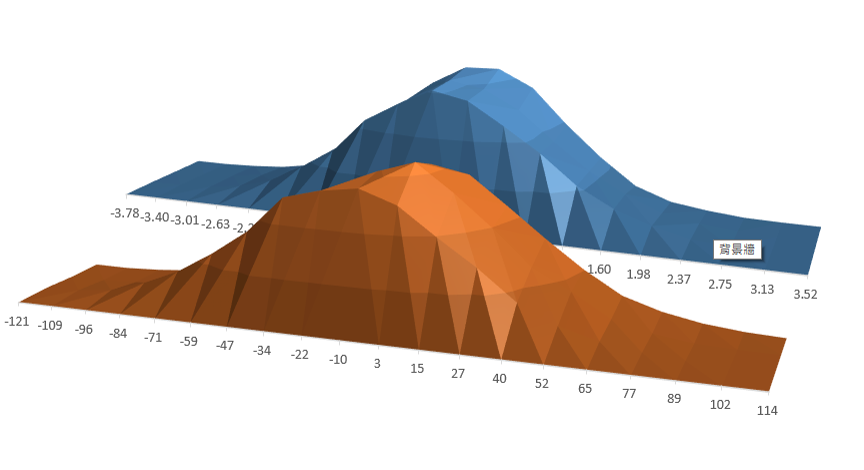
\includegraphics[width=1\linewidth]{inc/3_low_numeric_convolution_neural_network/figure/nor_dist.png}
    \caption{Given a threshold, calculate the error between reconstructed distribution and the original.}
    \label{fig:th_choice}
\end{figure}
\begin{table}[h]
    \caption{Threshold for each bit setting by $L_1$ norm error}
    \label{tab:threshold}
    \centering
    \footnotesize 
        \begin{tabular}{c|ccccccccc}
        \toprule
            Bit length &1 & 2 & 3 & 4 & 5 & 6 & 7 & 8 & 32 \\
            Threshold &1.2 & 1.9& 2.4& 2.7& 3.1& 3.5& 3.6& 3.7& 100 \\
 
        \bottomrule
        \end{tabular}
\end{table}

\section{Computational consideration and data re-packing}
Now that we have the quantized model, we need efficient computational strategy. Simply store the model, say quantized to 4 bits, in original 32-bit data type is 8x waste of storage, memory bandwidth and can't be effectively deployed to processing unit. We propose a simple data re-packing method, to tightly compact the data. However the compacted data requires specially designed processor to reach its full performance potential. Since we're aiming at large image recognition task, the data usually can't fit onto the accelerator entirely. We use several tiling parameters to split data into chunks and process them one at a time.
\subsection{Data re-packing}
We first determine a desirable MAC bit-length configuration \textbf{$A_b$}, usually the smaller bit-length of input and weight tensor. We then split each data point and distribute them to an additional tensor dimension \textit{bit channel} if the data bit-length is larger than \textbf{$A_b$}, \textbf{$X_b,W_b,O_b$} for input, weight, output respectively, note that \textbf{$O_b$} is dependent on the \textbf{$A'_b$} of the next layer. Say we are going to process a layer using 4-bit multiplication, \textbf{$A_b$} is chosen to be 4; in \autoref{fig:re_pack1}, original 4-bit data stored in wasteful 16-bit is re-packed along the \textbf{channel} dimension into new channel size of $C/4$; \autoref{fig:re_pack2} re-packs 8-bit data with additional \textbf{$X_b$} dimension of size 2.The re-packed data is meant to be added up within itself, and the data with different \textit{bit channel} bear different weighting of $2^{X_b*A_b}$. In the example, we need a arithmetic unit capable of summing up 4 4-bit multiplication within a 16-bit data, we call this \textbf{\textit{subword accumulation}} arithmetic dataflow, in contrast to the \textit{subword parallelism} dataflow where multiple output registers are needed, only one output register is needed at a time. We will elaborate in \autoref{ch:arch}.
\\
Having the data prepared through quantization and re-packing, we are ready to move on to the accelerator architecture designed for such data.
\begin{figure}
    \centering
    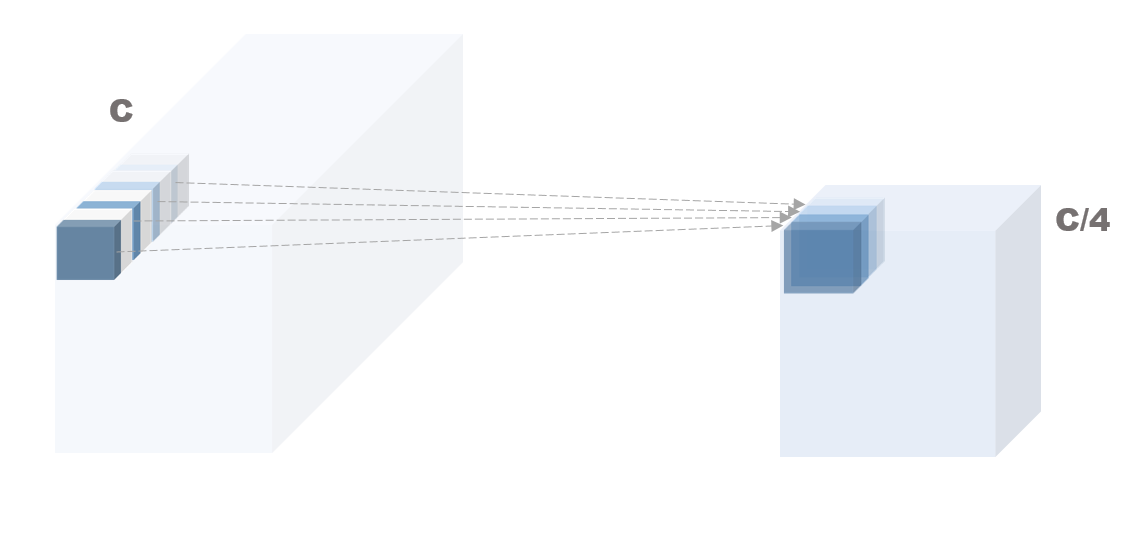
\includegraphics[width=1\linewidth]{inc/3_low_numeric_convolution_neural_network/figure/re_pack1.png}
    \caption{4-bit data repacked to 16-bit compact data.}
    \label{fig:re_pack1}
\end{figure}
\begin{figure}[h]
    \centering
    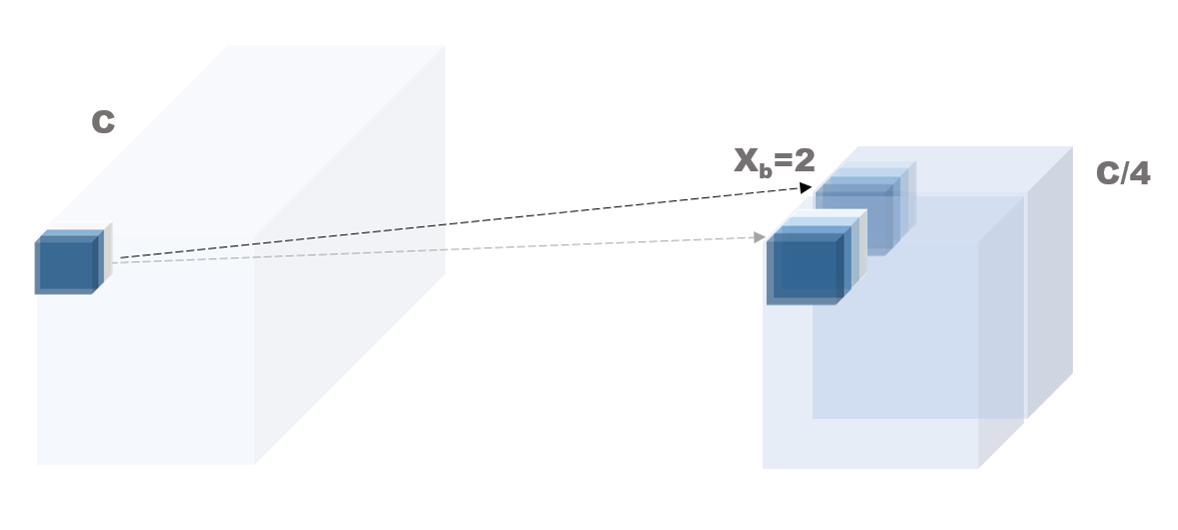
\includegraphics[width=1\linewidth]{inc/3_low_numeric_convolution_neural_network/figure/re_pack2.png}
    \caption{8-bit data repacked to 16-bit compact data with additional bit channel data of size 2.}
    \label{fig:re_pack2}
\end{figure}
\begin{table}[h]
    \caption{Low bit arithmetic and shape parameters}
    \label{tab:bit_shape}
    \centering
    \footnotesize 
        \begin{tabular}{cc}
        \toprule
        Parameter & Description \\
        \midrule
        $X_b$ & Input bit channels\\
        $W_b$ & Weight bit channels\\
        $O_b$ & Output bit channels\\
        $A_b$ & Arithmetic bit length\\
        $A'_b$ & Arithmetic bit length of the next layer\\
        \bottomrule
        \end{tabular}
\end{table}


\iffalse
    \begin{itemize}
    \textcolor{purple}{What knowledge is necessary to}
        \item \textcolor{purple}{understand design decisions you made, e.g. how did you choose the quantisation     algorithm?}
        \item \textcolor{purple}{understand why your research question is important, e.g. why should we quantise     CNNs?}
    \end{itemize}
\fi